%**VARIABILI PROGETTO DA MODIFICARE****************************

\def\PROJECT			{F1.js} %Nome del documento, ad esempio: Piano di Progetto
%Personale
%se ci sono più persone da indicare scrivere: {nome1, \\&nome2, \\&nome3 ecc..}
\def\AUTHOR			{\ME}
\def\REPOurl		{https://github.com/filnik/F1.js}

%Variabili documento
\def\TABLES		{false} %abilita - disabilita l'indice delle tabelle
\def\FIGURES	{true} %abilita - disabilita l'indice delle figure

%importa la struttura principale
\documentclass[a4paper,11pt]{article}

%Non modificare
\def\EMAIL			{filnik90@gmail.com}
\def\ME				{\mbox{Filippo De Pretto}}
\def\SERIAL			{\mbox{610673}}
\def\SUPERVISOR		{\mbox{Mauro Conti}}
\def\TUTOR			{\mbox{Fabio Aiolli}}
\def\END			{Padua, Italy, 2012.}

%*****nuovi comandi************************
%fornisce il caption per riferirsi ad una particolare sezione
\newcommand{\numref}[1]{\textsf{[\ref{#1}]}}
%formattazione per il glossario
\newcommand{\gl}[1]{\underline{#1}}
%**IMPORTAZIONE PACKAGE**************************
\usepackage[italian, english]{babel}
\usepackage[utf8]{inputenc}
\usepackage[T1]{fontenc}
\usepackage{graphicx}
\usepackage{float}
\usepackage{tabularx, array}
\usepackage{longtable}
\usepackage{chapterbib}
\usepackage[a4paper,top=3cm,bottom=3cm,left=3cm,right=3cm,bindingoffset=5mm]{geometry}
\usepackage[colorlinks=true, urlcolor=blue, citecolor=black, linkcolor=black]{hyperref}
\usepackage{booktabs}
\usepackage{totpages}
\usepackage{dcolumn}
\usepackage{epstopdf}
\usepackage{booktabs}
\usepackage{fancyhdr}
\usepackage{calc}
\usepackage{datatool}
\usepackage{listings}
\usepackage{url}
\usepackage{hyperref}
\usepackage{fancyhdr}
\usepackage{color}
\usepackage{wrapfig}

\usepackage{caption}
\usepackage{subcaption}

\definecolor{lightgray}{rgb}{.9,.9,.9}
\definecolor{darkgray}{rgb}{.4,.4,.4}
\definecolor{purple}{rgb}{0.65, 0.12, 0.82}

\lstdefinelanguage{JavaScript}{
  keywords={typeof, new, true, false, catch, function, return, null, catch, switch, var, if, in, while, do, else, case, break},
  keywordstyle=\color{blue}\bfseries,
  ndkeywords={class, export, boolean, throw, implements, import, this},
  ndkeywordstyle=\color{darkgray}\bfseries,
  identifierstyle=\color{black},
  sensitive=false,
  comment=[l]{//},
  morecomment=[s]{/*}{*/},
  commentstyle=\color{purple}\ttfamily,
  stringstyle=\color{red}\ttfamily,
  morestring=[b]',
  morestring=[b]"
}

\lstset{
   language=JavaScript,
   backgroundcolor=\color{lightgray},
   extendedchars=true,
   basicstyle=\footnotesize\ttfamily,
   showstringspaces=false,
   showspaces=false,
   numbers=left,
   numberstyle=\footnotesize,
   numbersep=9pt,
   tabsize=2,
   breaklines=true,
   showtabs=false,
   captionpos=b
}

\frenchspacing % correct spaces
\def\SCOPOPROD		{The goal of the project \gl{\PROJECT{}} is to develop an Android Application to collect informations about cellphone usage to develop new trasparent authentication method using that data.}
%**STILE PAGINA**********************************

\pagestyle{fancy}

%no indentazione paragrafo
%\setlength{\parindent}{0pt}

%intestazione
\lhead{\Large{\PROJECT{}}}
%\rhead{\includegraphics[keepaspectratio = true, width = 30px] {images/gufyIcon.png}}
\renewcommand{\headrulewidth}{0.4pt}  %Linea sotto l'intestazione
%\headsep = 35px

%piè di pagina
%\lfoot{\footnotesize{{mailto:\EMAIL}{\EMAIL}}}
\rfoot{\thepage} %per le prime pagine: mostra solo il numero romano
\cfoot{}
\renewcommand{\footrulewidth}{0.4pt}   %Linea sopra il piè di pagina

%**PRIMA PAGINA ***************************

\begin{document}		
%Prima pagina senza intestazione né piè di pagina									
\thispagestyle{empty}

%Centra il testo
\begin{center}
%\vspace{1cm}

%Titolo del PROJECT

\includegraphics[height=120px]{../documentation/img/unipd_logo.png}

\vspace{0.5cm}
{\Huge University of Padova}\\[.5pc]
{\Large Department of Mathematics}\\[.5pc]
\vspace{5 mm}
{\Huge \textbf{\PROJECT{}}}\\[.5pc]
{\Huge \SUBTITLE}\\[.4pc]
{\Large Project for BS Degree in Computer Science}\\[.5pc]
{\Large \emph{\ME{} - student number: \SERIAL{}}}\\[1pc]

%\includegraphics[height=120px]{images/gufyIcon.png}

\vspace{0.5cm}
{\Large \END}\\[3pc]

%Tabella con informazioni documento. Le seguenti variabili devono essere definite
%nel file .tex che include questa struttura
\normalsize{
	\begin{tabular}{r|l}
		\multicolumn{2}{c} {\textbf{Informations about the document}} \\
		\midrule
		\textbf{Author} 				& \AUTHOR \\
		\textbf{Supervisor} 			& \SUPERVISOR \\
		\textbf{Internal tutor} 		& \TUTOR \\
	\end{tabular}
}

%Fine zona centrata
\end{center}

%Indica che è finita la pagina corrente ed inizia la prossima
\newpage
%si usa la numerazione romana per gli indici e la tabella delle modifiche
\pagenumbering{Roman}
%************************************************


\newpage
%************************************************
%importa i vari indici
%************************************************
%Inserisce il link all'indice
\addcontentsline{toc}{section}{Index}
\tableofcontents
\newpage

%se è stata impostata a true la variabile per la lista delle tabelle, la mostra
\ifthenelse{\equal{\TABLES}{true}} 
{\listoftables \newpage}{}

%se è stata impostata a true la variabile per la lista delle figure, la mostra
\ifthenelse{\equal{\FIGURES}{true}}
{\listoffigures \newpage}{}

%da qui comincia la numerazione normale
\pagenumbering{arabic}

%imposta il formato di visualizzazione
\rfoot{\thepage ~of~\pageref{TotPages}}

%**********   Inizio delle "section"   ********************************

\newpage

\begin{center}
\section*{Abstract}
\end{center}
In this document is described how the F1.js program has been designed and implemented. It is a project developed for the ``Concurrent and distributed systems'' exam, matching the requirements that can be found at: \url{http://www.math.unipd.it/~tullio/SCD/2008/Progetto.html}

 The programming language chosen for this project is Javascript/node.js, for its particular properties that makes this task a lot easier than in other languages.

This is accomplished by the fact that in node.js there is no difference between concurrency and distribution, as it will be explained.

\newpage
\section{The language}
In order to understand how we solved the problem, is important to give an explanation of how the language, its architecture and its tools are designed. Indeed, this is not a common architecture, although there are similar examples such as Twisted for Python or Event Machine for Ruby.

\subsection{node.js features}

As said, the project has been written using node.js. Quoting the official site's main page: \textit{Node.js is a platform built on Chrome's JavaScript runtime for easily building fast, scalable network applications. Node.js uses an event-driven, non-blocking I/O model that makes it lightweight and efficient, perfect for data-intensive real-time applications that run across distributed devices.}\footnote{Official node.js website: \url{http://www.nodejs.org}}

In other words, it is expressive, in particular with the Express.js framework\footnote{Official Express.js framework website: \url{http://expressjs.com/}}, fast and scalable. 

An important aspect is the use of the V8 JavaScript Engine to interpret the JavaScript code. Written by Google, it increases performance by compiling JavaScript to native machine code (x86, ARM, or MIPS CPUs)\cite{website:v8-intro}, before executing it, versus executing bytecode or interpreting it.

As you can see in Figure \ref{fig:nodeBench}, this raises a lot the performances, reaching almost Java's speed.

\begin{figure}[H]
\centering % per centrare l'immagine (opzionale)
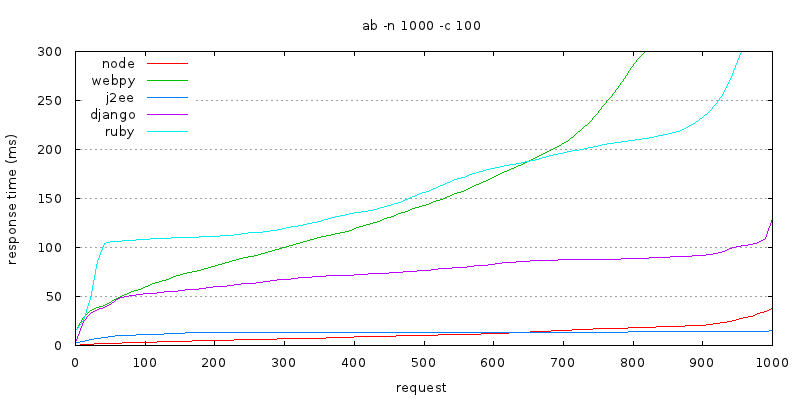
\includegraphics[height=150px]{img/node-bench.png}
\caption{node.js benchmark versus other popular languages/platforms/frameworks}
\label{fig:nodeBench}
\end{figure}

However, the performance aren't great only for the use of V8, but also for the programming style that node.js implies.

\subsubsection{Asynchronous I/O}
\label{sec:async}

node.js real difference is the asynchronous I/O and evented support. Citing ``cloudfoundry.com'' \cite{website:cloudfoundry}: \textit{In order to write a fast and scalable server application, we typically end up writing it in a multi-threaded fashion. While you can build great multi-threaded apps in many languages, it usually requires a lot of expertise to build them correctly. On the other hand, these libraries (along with Chrome’s V8 engine) provide a different architecture that hides the complexities of multi-threaded apps while getting the same or better benefits.}

\textit{Let's compare classic multi-threaded server with an evented, non-blocking I/O server:}

\begin{figure}[H]
\centering % per centrare l'immagine (opzionale)
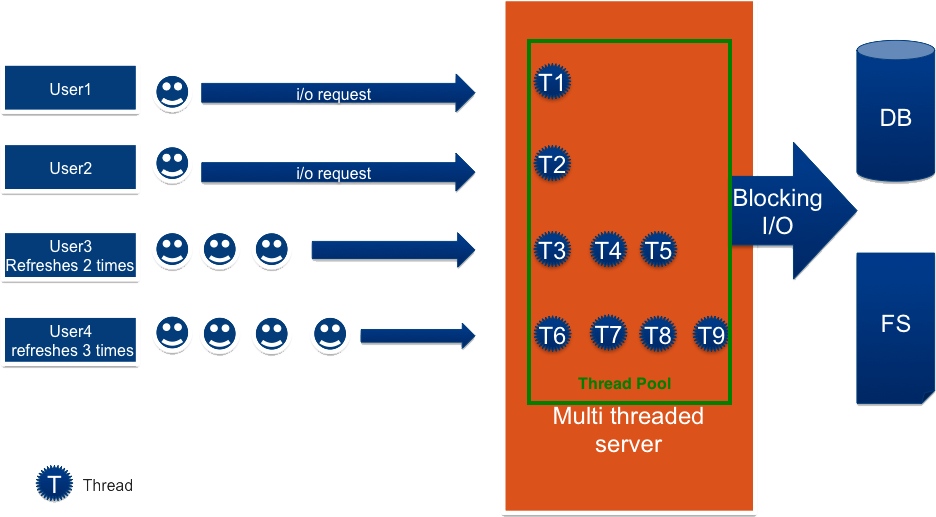
\includegraphics[height=150px]{img/multiThreadedServer.png}
\caption{An example multi-threaded HTTP server using blocking I/O}
\label{fig:multiThreadedServer}
\end{figure}

\textit{The diagram in Figure \ref{fig:multiThreadedServer} depicts a simplified multi-threaded server. There are four users logging into the multi-threaded server. A couple of the users are hitting refresh buttons causing it to use lot of threads. When a request comes in, one of the threads in the thread pool performs that operation, say, a blocking I/O operation. This triggers the OS to perform context switching and run other threads in the thread pool. And after some time, when the I/O is finished, the OS context switches back to the earlier thread to return the result.}

\textit{\textbf{Architecture Summary:} Multi-threaded servers supporting a synchronous, blocking I/O model provide a simpler way of performing I/O. But to handle a heavy load, multi-threaded servers end up using more threads because of the direct association to connections. Supporting more threads causes more memory and higher CPU usage due to more context switching among threads.}

\begin{figure}[H]
\centering % per centrare l'immagine (opzionale)
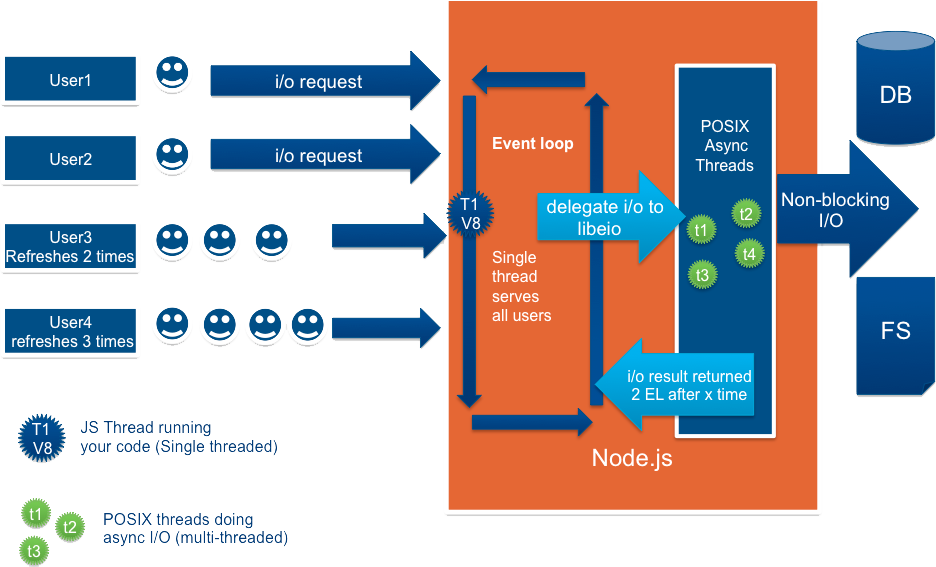
\includegraphics[height=150px]{img/NodeJS-EventedIOAsyncIO_latest.png}
\caption{Event-driven, non-blocking I/O (Node.js server)}
\label{fig:nodejsServer}
\end{figure}

\textit{The diagram in Figure \ref{fig:nodejsServer} depicts how Node.js server works. At a high level, Node.js server has two parts to it:}
\begin{itemize}
\item \textit{At the front, you have Chrome V8 engine (single threaded), event loop and other C/C++ libraries that run your JS code and listen to HTTP/TCP requests;}
\item \textit{And at the back of the server, you have libuv (includes libio) and other C/C++ libraries that provide asynchronous I/O.}
\end{itemize}

\textit{Whenever a request is made from a browser, mobile device, etc., the main thread running in the V8 engine checks if it is an I/O. if it is an I/O then it immediately delegates that to the backside (kernel level) of the server where one of the threads in the POSIX thread pool actually makes async I/O. Because the main thread is now free, it starts accepting new requests/events.}

\textit{And at some point when the response comes back from a database or file system, the backend piece generates an event indicating that we have a result from I/O. And when V8 becomes free from what it is currently doing (remember it is single-threaded), it takes the result and returns it to the client.}

\textit{\textbf{Architecture Summary:} This architecture utilizes an event loop (main thread) at the front and performs asynchronous I/O at the kernel level. By not directly associating connections and threads, this model needs only a main event loop thread and many fewer (kernel) threads to perform I/O. Because there are fewer threads and consequently less context-switching, it uses less memory and also less CPU.}

\subsection{Concurrency and distribution in node.js}

We have seen why an asynchronous webserver is a lot faster than a synchronous one. The fact is that performances might not be so interesting, as in this situation, but might be more interesting the easiness of designing and implementing the solution.

As said concurrency and distribution in node.js are the exact same thing. The reality indeed is that node.js is (mainly) single-threaded as seen before, handling everything with events. For this reason there isn't the concept of ``lock'' in node.js or of threads. It's possible to use webworkers that are processes that you can create forking the single-thread but are heavy and usually not needed, like in this case. They are needed only in cases of CPU-intensive tasks that might block the main thread from answering the events that it gets.

So, when you have the application that waits for an event, it's of no importance to know if the event is generated in the client, in the server or in another server. The important thing is to be subscribed to the right event emitter, and this can be easily done and changed, even at run-time.

In this way, we can run the program in a single instance on a server, in multiple processes in a single server or even split the processes in different servers without affecting the logic of the application at all. This means that we can partition vertically every single event emitter, if we want. This is a lot more scalable than rewriting the whole application or to adapt it in both cases.

\subsection{node.js versus Twisted and Event Machine}

Basically the great advantage of node.js is the use of the JavaScript language. The reason is that all the libraries already written for the JavaScript language are asynchronous, since it's how JavaScript has been designed, while Python and Ruby have a lot of synchronous libraries that you cannot use inside these two asynchronous environments.

Another important fact is that now JavaScript is an isomorphic language.\textit{By isomorphic we mean that any given line of code (with notable exceptions) can execute both on the client and the server.}\cite{website:isomorfic}

This seems trivial but it's not. Indeed we can easily communicate between client and server in a single language using events and, if needed, RPC. We can indeed write the same library for the client and the server and validate the data in each step to prevent code changes. We have no mind-switch from one language to another and the application can avoid to decouple in a strictly way view from controller from model, since the client-server limit is not so strict as in other contexts.

\subsection{socket.io, ascoltatori and redis}

\begin{figure}[H]
\centering % per centrare l'immagine (opzionale)
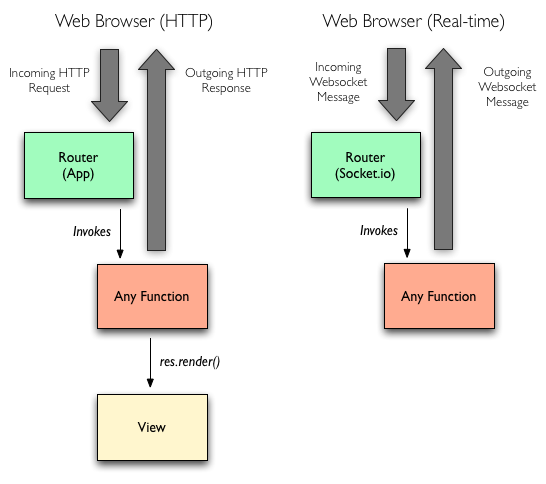
\includegraphics[height=250px]{img/express.png}
\caption{Express and socket.io model}
\label{fig:expressSocketio}
\end{figure}

In Figure \ref{fig:expressSocketio} you can see how the framework used and socket.io work. They are really simple and neat. Express has only the job to answer the web requests and render the HTML pages. Socket.io is a wrapper over the websocket technology.

\textbf{Socket.io} solves a lot of problems that occurs if you use the websocket technology as it is. What socket.io handles is:
\begin{itemize}
\item the connection. Websocket is a modern technology that is not available in old browsers. This library overcomes this problem using different technologies using the fastest possible. In this way it degradates gracefully from Websocket to Flash or even the AJAX long-polling technology;
\item the re-connections without creating different instances but reusing the same instance that there were before the disconnection;
\item the send of JSON objects instead of plain text;
\item the namespaces. In this way you can have a single websocket connection but using different namespaces to divide different parts of the logic.
\end{itemize}

In this way, we are totally unaware of the underlining problems of the network and we can handle the problem in a lot easier way.

It allows you also to pass pointers to functions that are executed in the context of definition. In this way you can simulate a Remote Procedure Call, if needed, without loosing transparency at all since it's all asynchronous. In this way, you don't need to handle problems regarding the proxy/skeleton pattern.

\textbf{Ascoltatori} is another really useful wrapper library. It is really interesting since it makes a lot easier and transparent the communication server to server. Indeed it wraps a lot of ways to communicate, in particular: Redis, AMPQ (RabbitMQ), ZeroMQ, MQTT (Mosquitto) or just plain node.js.

In this way, we can have for example a node of the network written in C++ with ZeroMQ and use this library to make everything work without changing a line of code.

We choose \textbf{Redis} because it ``is a database, but it would be more accurately described as a datastructure server'' \cite{book:smashing}. In this way we can use only one technology both for communication and storage. Instead of setup a Redis instance, we choose to use redistogo, that is an online storage service (it would work in local too, anyway).

\section{The problem}
\label{sec:theProblem}

To analyse the problem we have chosen to describe it through UML-schemas in order to have a clear path to follow.

\subsection{F1.js}

\begin{figure}[H]
\centering % per centrare l'immagine (opzionale)
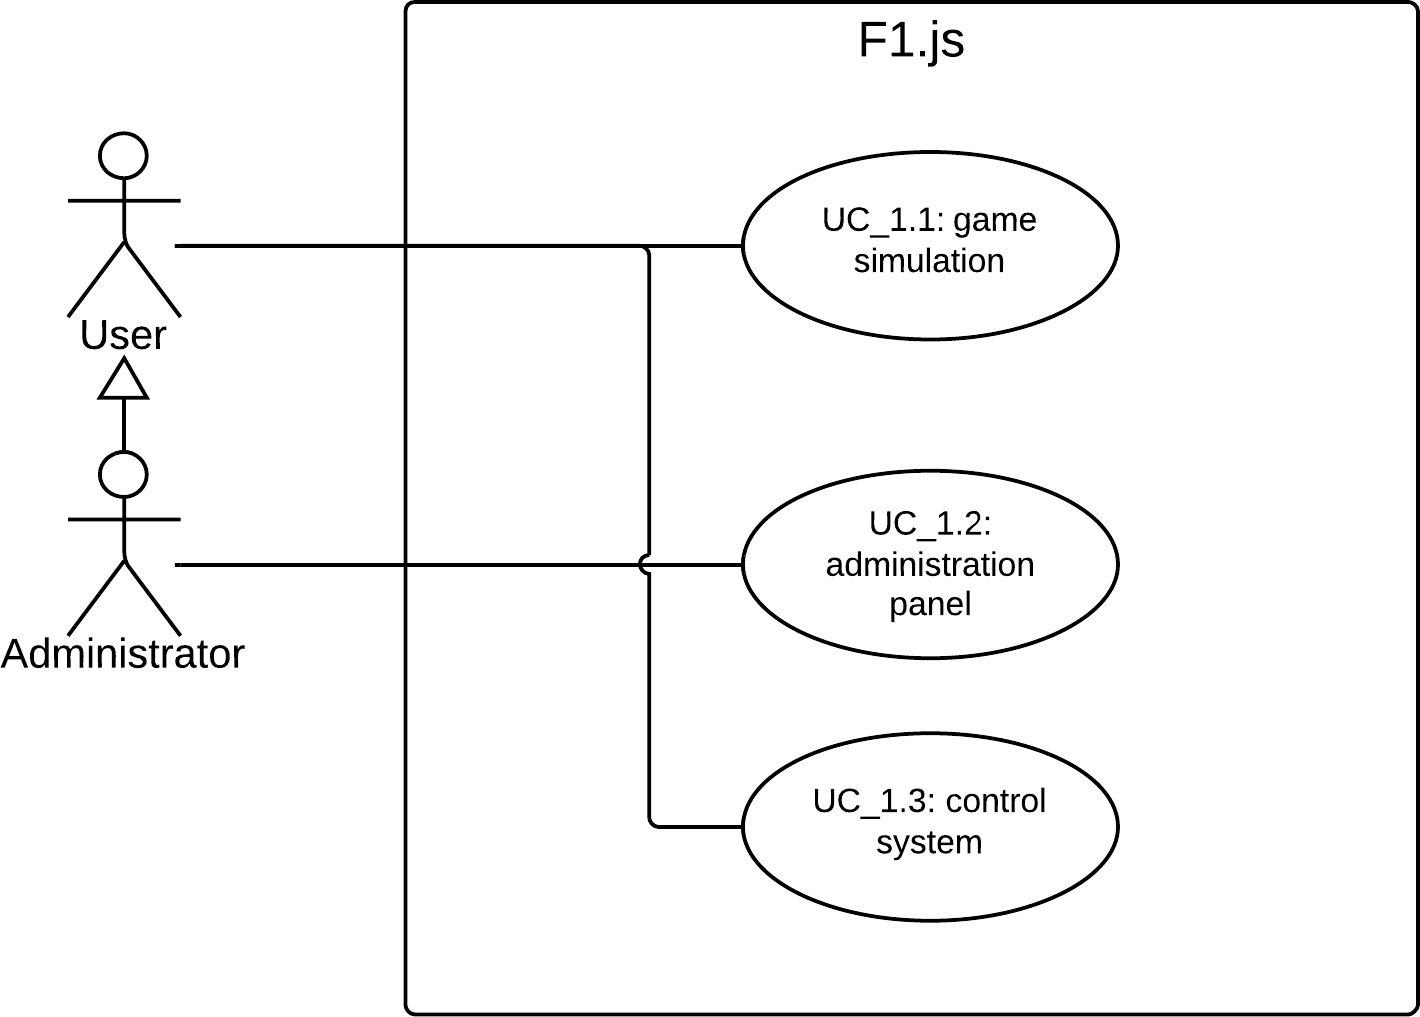
\includegraphics[height=250px]{./img/UML/F1Js.png}
\caption{F1.js - the system}
\label{fig:F1jsUC}
\end{figure}

In Figure \ref{fig:F1jsUC} is described the problem divided in its 3 main parts: the game simulation, the administration panel and the control system.

The normal user can enter the game simulation and view the control system with the status of the simulation. Only the administrator can change some of the game settings.

\subsection{The Game Simulation}

\begin{figure}[H]
\centering % per centrare l'immagine (opzionale)
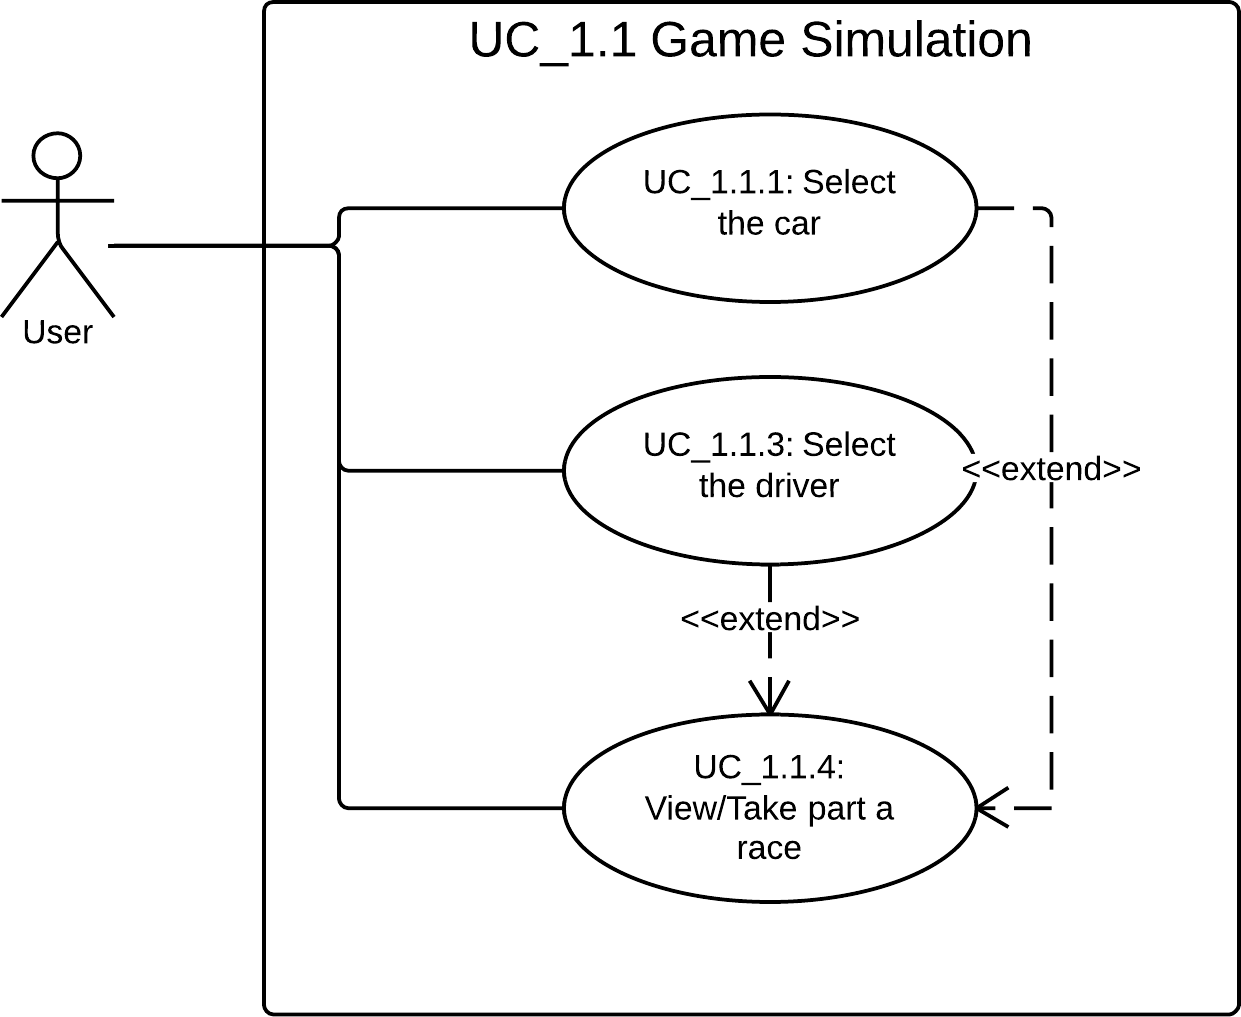
\includegraphics[width=0.6\textwidth]{./img/UML/GameSimulation.png}
\caption{The Game Simulation}
\label{fig:GameSimulation}
\end{figure}

When a new user connects to the system, she can decide what car and which player to play with. If she doesn't want, she can let the default parameters. Finally, she can decide to view or to take part to the current race. If there are already enough player, the race begins and every new player can only watch the competition.

\subsection{The Administration Panel}

\begin{figure}[H]
\centering % per centrare l'immagine (opzionale)
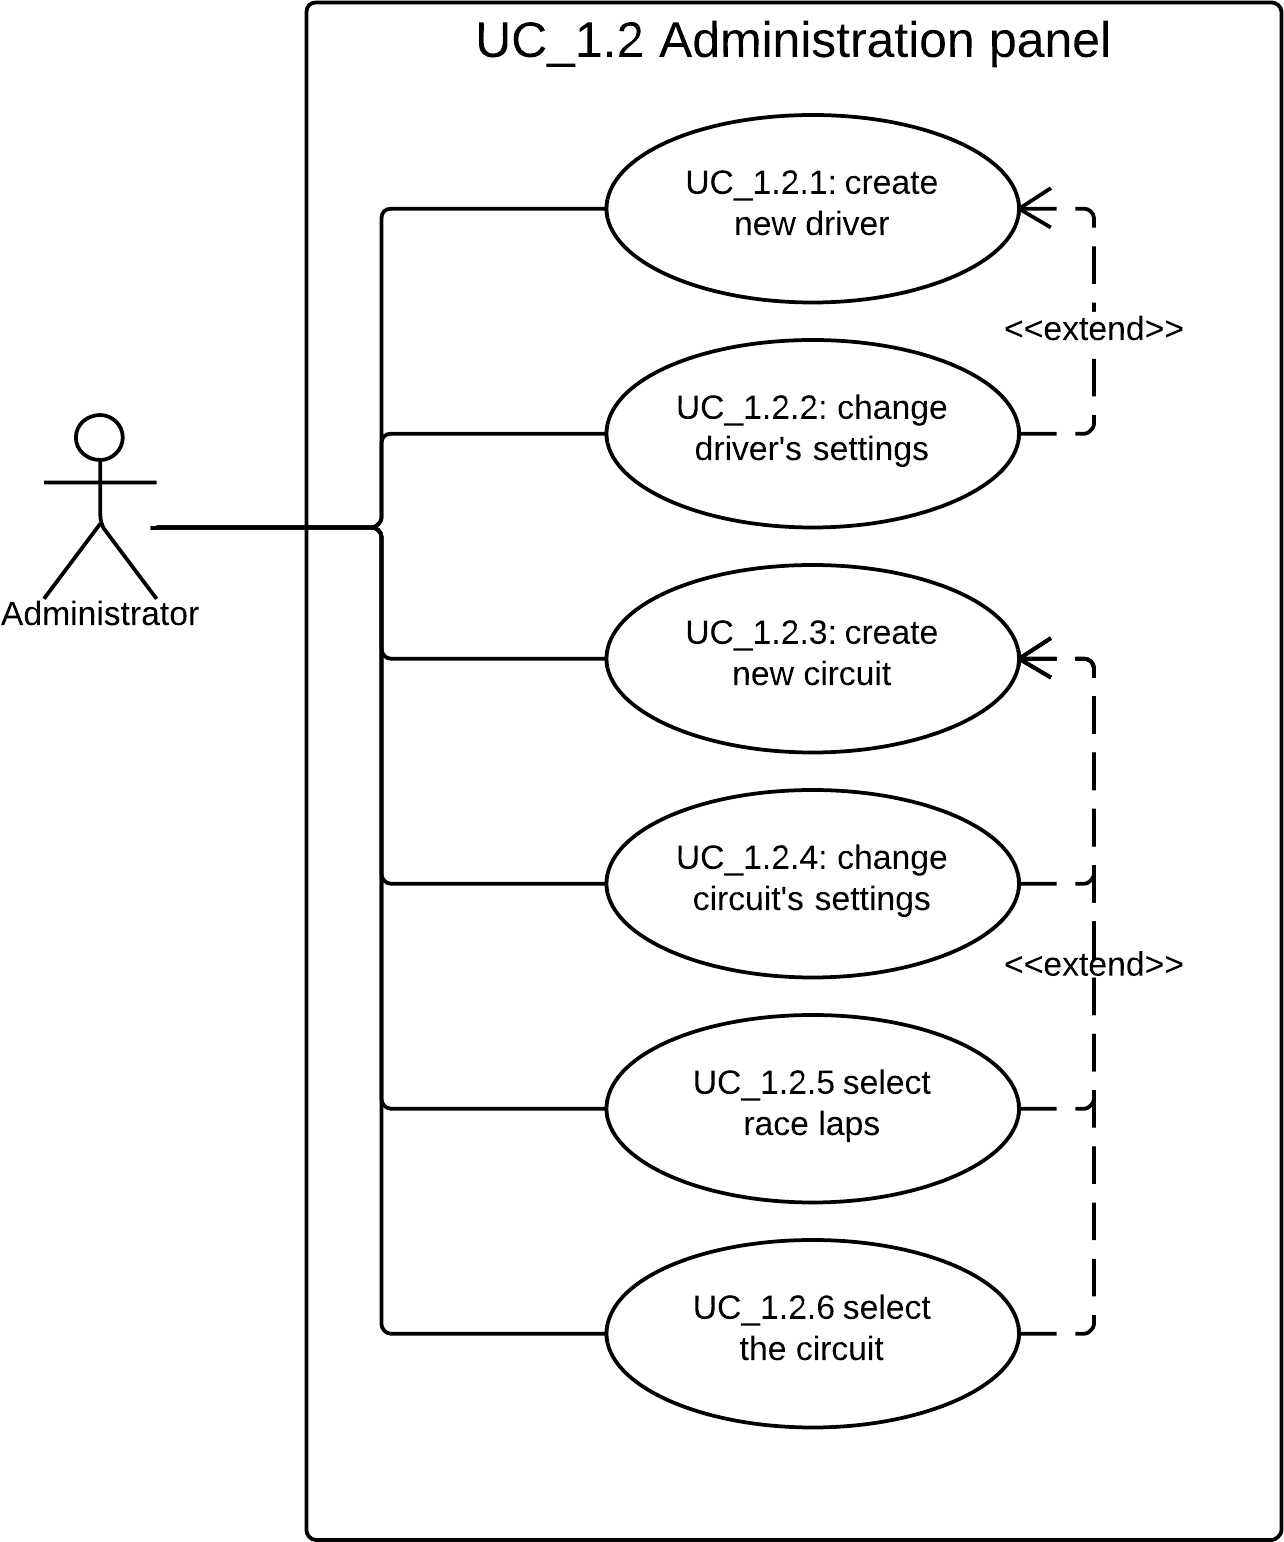
\includegraphics[width=0.6\textwidth]{./img/UML/AdministrationPanel.png}
\caption{The Administration Panel}
\label{fig:AdministrationPanel}
\end{figure}

In Figure \ref{fig:AdministrationPanel} there is the panel where the administrator can change some parameters of the simulation. The administrator can:
\begin{itemize}
\item create a new driver or change the parameters of an old one;
\item create a new circuit or change the parameters of a circuit already inserted;
\item select the race laps for the next race;
\item select the circuit of the next race.
\end{itemize}

\subsection{The Control System}

\begin{figure}[H]
\centering % per centrare l'immagine (opzionale)
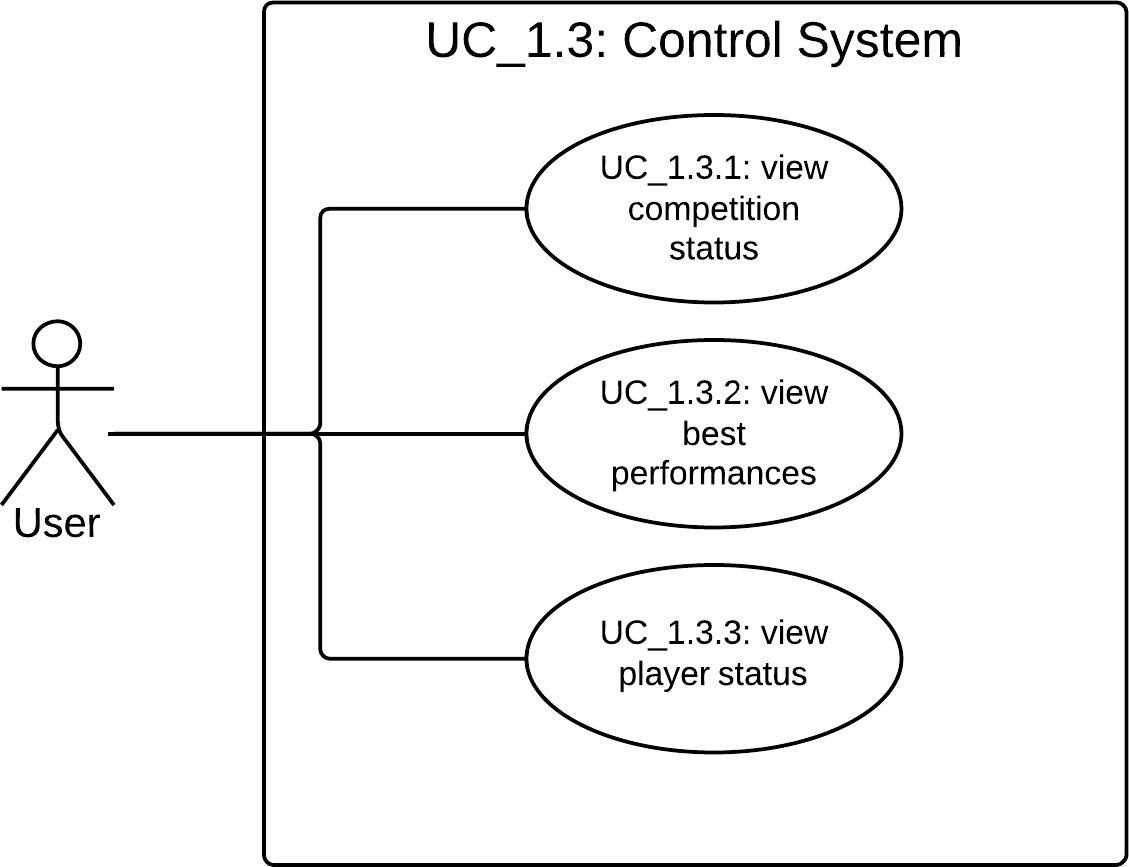
\includegraphics[width=0.6\textwidth]{./img/UML/ControlSystem.png}
\caption{The Control System}
\label{fig:ControlSystem}
\end{figure}

In Figure \ref{fig:ControlSystem} is described the control system. Every user can view:
\begin{itemize}
\item the competition's status;
\item the best performance until now;
\item the player's status.
\end{itemize}

\section{System Analysis}

\begin{figure}[H]
\centering % per centrare l'immagine (opzionale)
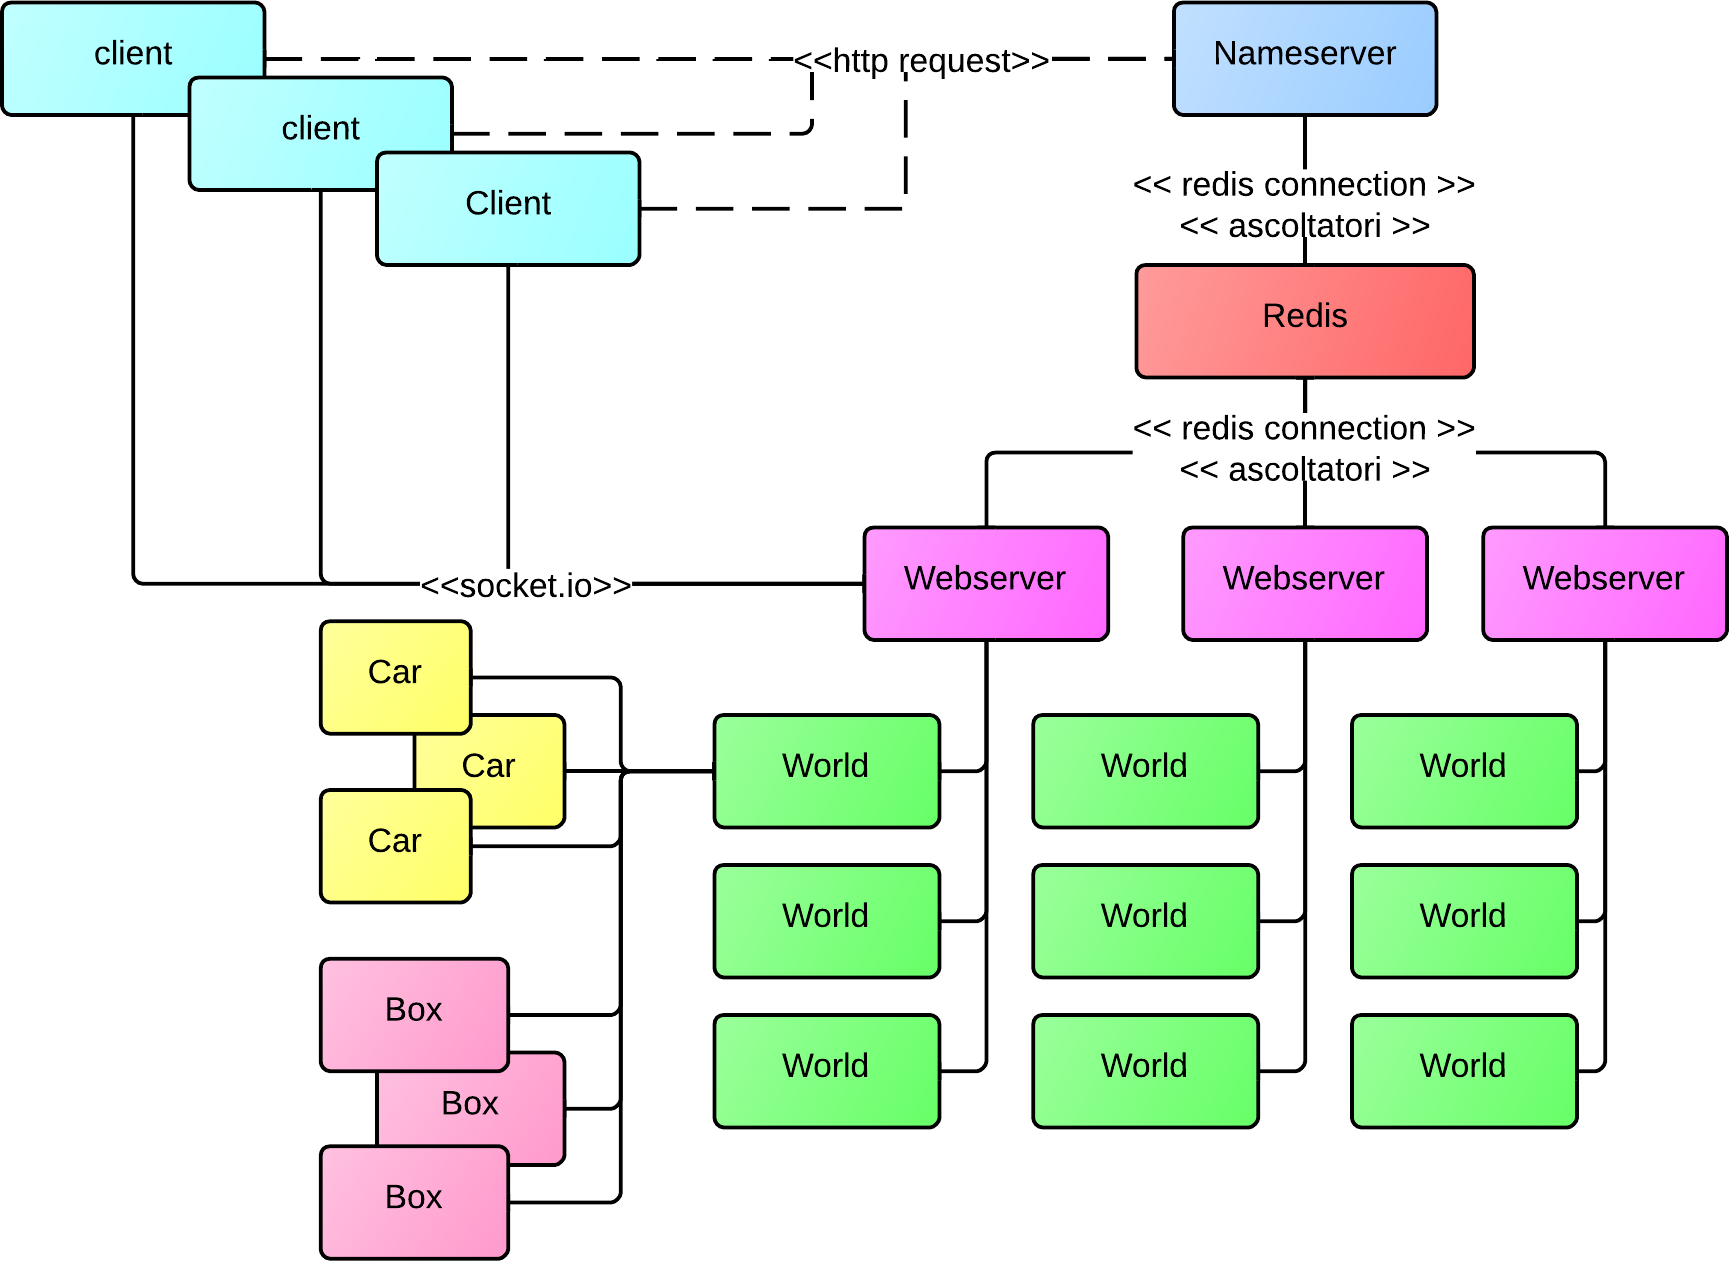
\includegraphics[width=0.8\textwidth]{./img/SystemAnalysis/Entities.png}
\caption{Main system's entities}
\label{fig:entities}
\end{figure}

In Figure \ref{fig:entities} is described the main system architecture proposed. There are some clients that connects through a web browser to the website and one, or more, servers that handle the requests.

\subsection{Client}

In our system, the clients are monitors and can do the action described in the use cases in Section \ref{sec:theProblem}. In the solution proposed they does nothing, they are only interfaces. They can indeed not communicate directly with other clients, due to the limitations of the JavaScript language. 

However, since the language is isomorphic, a whole simulation can be moved to one client and run there with all the parameters set previously. Obviously, that client will be the only monitor if there is not a server that works as a bridge for all the other clients. This situation is shown in Figure \ref{fig:entitiesMagicClient}, where a client simulates the whole system and returns the results to the other client.

\begin{figure}[H]
\centering % per centrare l'immagine (opzionale)
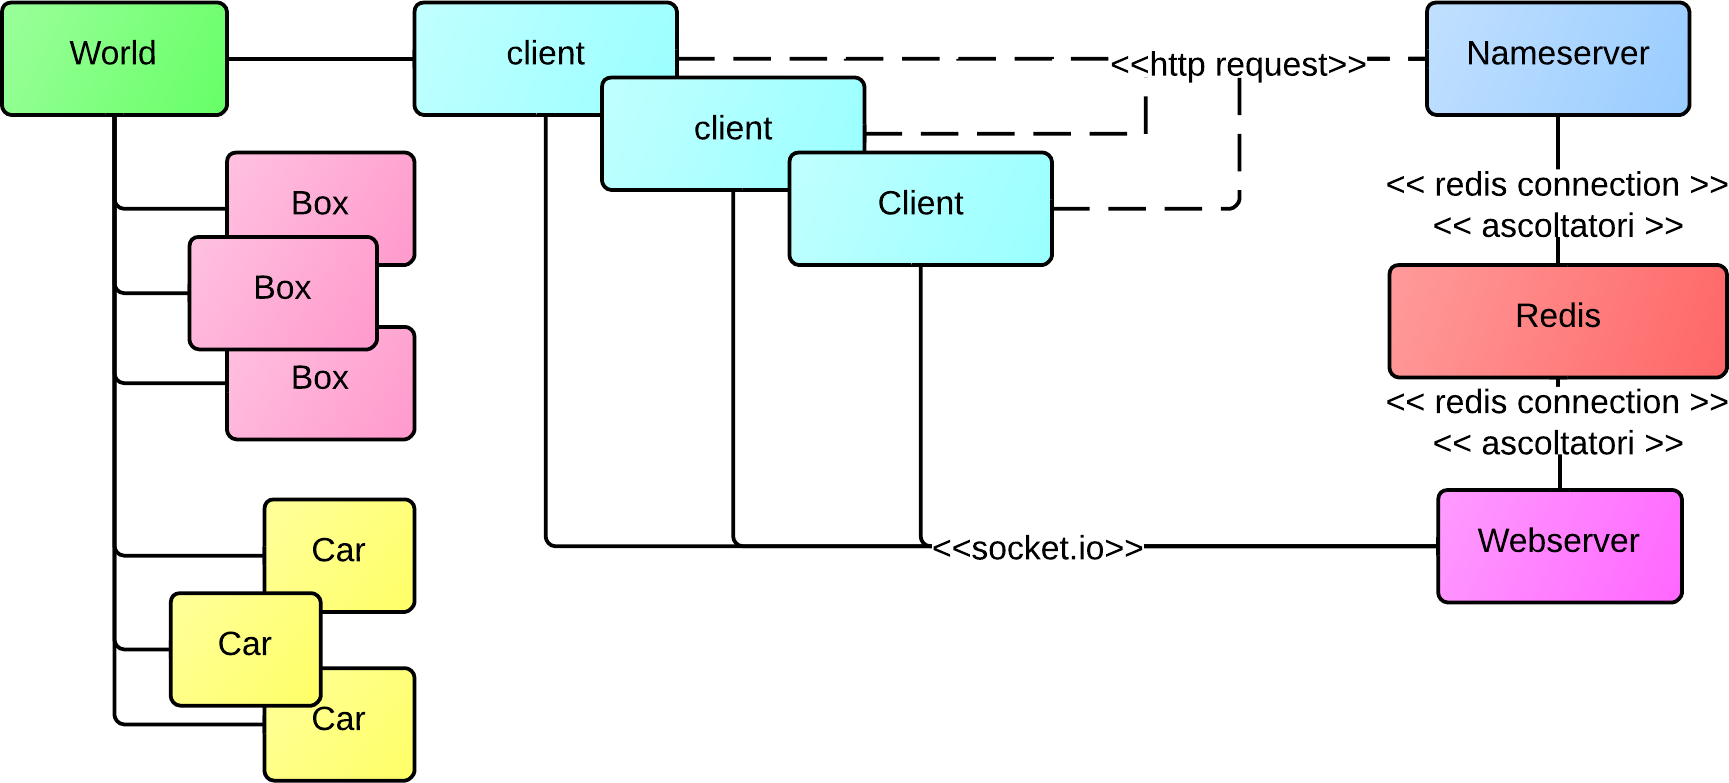
\includegraphics[width=0.8\textwidth]{./img/SystemAnalysis/EntitiesMagicClient.png}
\caption{Alternative vision of the system client-focused}
\label{fig:entitiesMagicClient}
\end{figure}

This solution, although may seem ``strange'' at first sight, is similar to the server-client architecture designed in some multiplayer games where one client acts as a server too. However, since the security issues and the increased overhead caused by the client-server-client communication, this choice hasn't been chosen. Although it would be really easy to switch, since you have only to move the code and redirect the calls.

\subsection{Nameserver}

In Figure \ref{fig:entities} you can see the we have chosen to have a nameserver too. The reason is because it servers as a name solver and a balancer too. We need to have an active figure that update the redis database with the entities that are connected to the system.

In this way, we can redirect every client call to the less loaded webserver and to let it join to the selected simulation .

Having only the redis instance operative, would lead to ghosts every time an entity disconnects itself, while in this situation the nameserver will keep the situation monitored.

\subsection{Redis}

\begin{figure}[H]
\centering % per centrare l'immagine (opzionale)
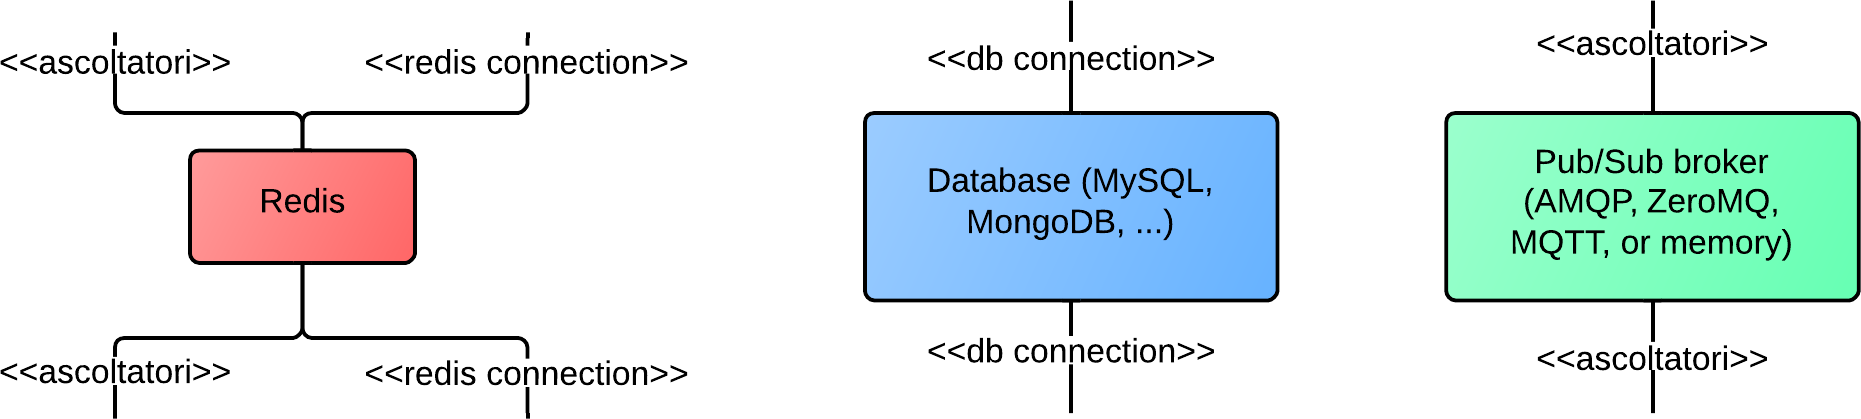
\includegraphics[width=0.8\textwidth]{./img/SystemAnalysis/RedisPubSubBroker.png}
\caption{Redis VS other solutions}
\label{fig:redisVSotherSolutions}
\end{figure}

For the reasons explained above Redis comes very handy for this use case. It serves indeed as a database and as a pub/sub broker too, that allows our server-to-server communications. The current solution is show in the left part of Figure \ref{fig:redisVSotherSolutions}. However, if we want, we can split the Redis entity in two (database+pub/sub broker) and handle the two jobs in a separate way, as you can see in the right part of Figure \ref{fig:redisVSotherSolutions}.

\subsection{Webserver}

\begin{figure}[H]
\centering % per centrare l'immagine (opzionale)
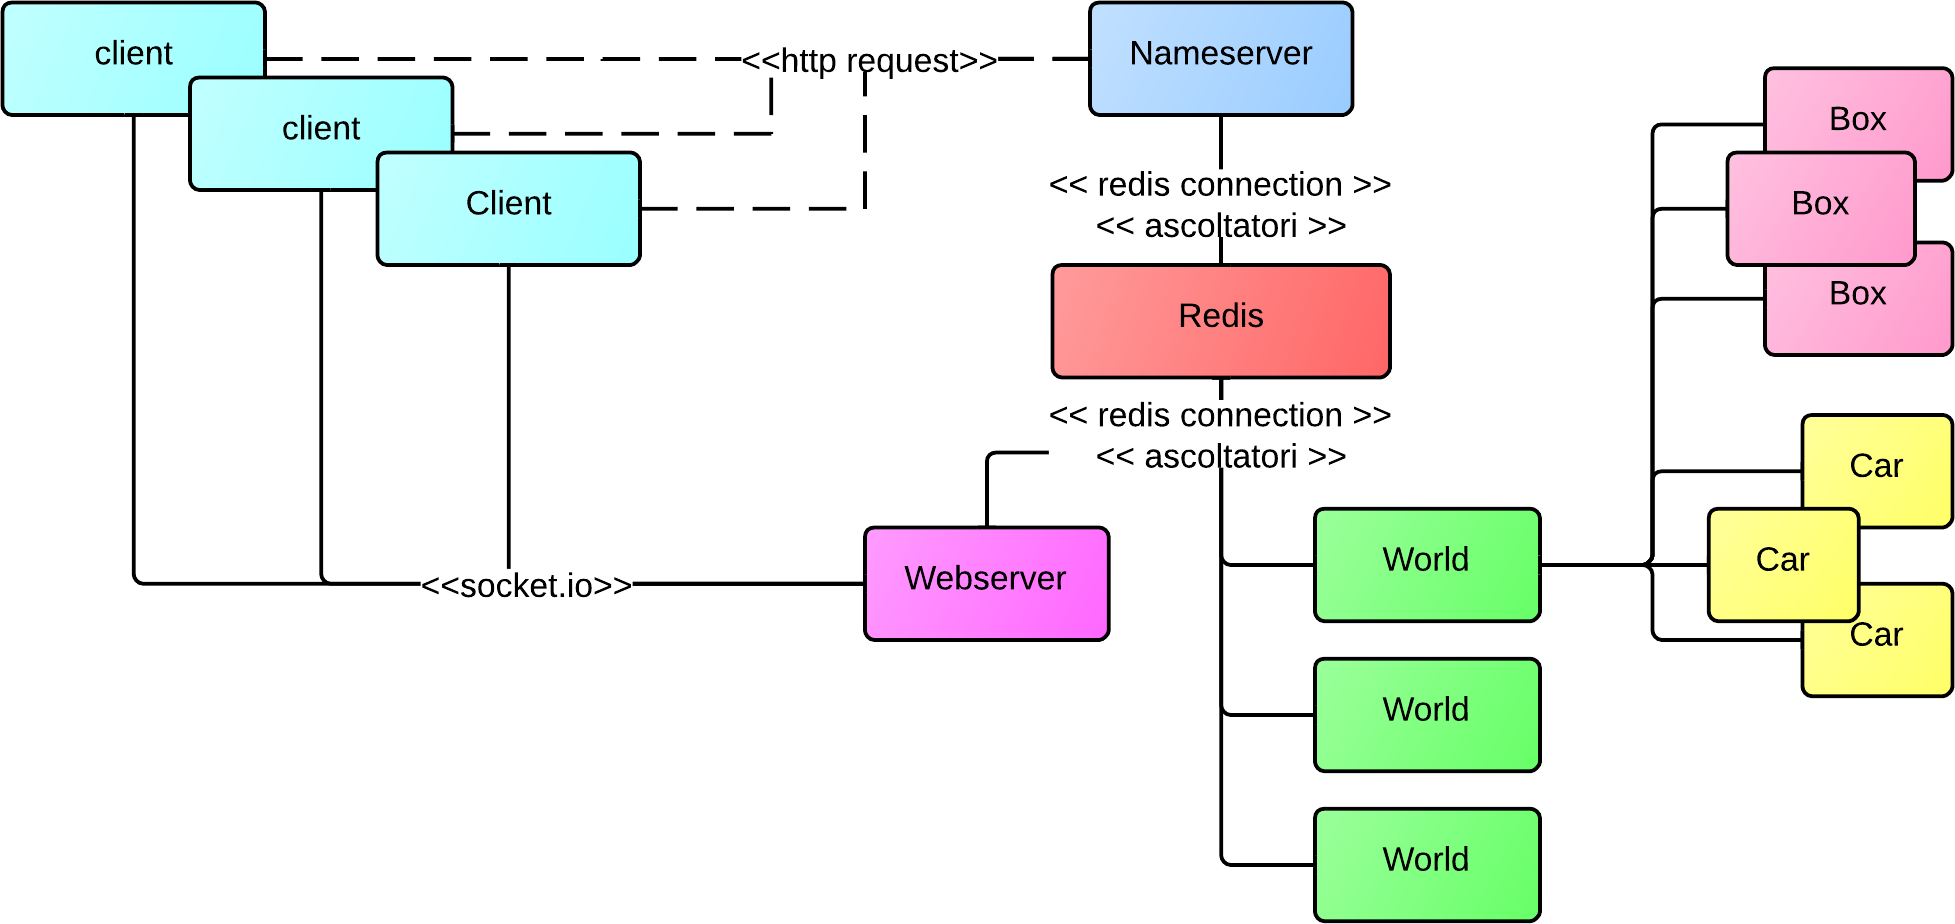
\includegraphics[width=0.8\textwidth]{./img/SystemAnalysis/EntitiesWebserver4everAlone.png}
\caption{Simulation separated from the Webserver}
\label{fig:entitiesWebserver4everAlone}
\end{figure}

In the architecture chosen as default (shown in Figure \ref{fig:entities}) there is only Client, Webserver, Redis and the Nameserver as active entities. This is because of the fact that there is no need of a further grade of distribution. As we know, more distribution will lead to possible lags, fragilities and problems. The system is also horizontally distributed, so if a webserver dies, the nameserver can redirect all the simulations to another one.

However, World, Car and Box can be distributed if needed, as you can see in Figure \ref{fig:entitiesWebserver4everAlone} (the other webservers are omitted in the Figure). The reason is pretty basic. Since they are event emitter, there is no need for them to be local, but they can be set everywhere they can be reached. Obviously the simulation will start with a bigger delay, there can be problems such a fault of the communication (or a disconnection of a box, for example), but you can choose this solution if you want it.

The webservers are not connected to each other since there is no need of communication. Every simulation is indeed atomic. We could however connect every webserver if we want to add the ability (not required) to move a live simulation from a webserver to another one. This could be easily done, since the whole simulation is a JSON object and the IA logic is shared in the webservers. So we would only have to add the ability for the clients to change the webserver with whom it is connected, that is pretty basic (simply send the address to the client and create a new socket.io connection, disconnecting from the previous one).

This can be easily done settings a flag, since the communication instead of being in the local memory, it occurs through Ascoltatori.

\subsection{World, Car, Box}

The World represents the circuit, the boxes, the cars and the players. As we have said, the world could be both on the server (Figure \ref{fig:entities}) or on the client (Figure \ref{fig:entitiesMagicClient}). It can be also distributed as a separate process on the same server or in another server at all. Since every parts of it are connected through Ascoltatori, every parts of it can be distributed easily to other servers.

We can decide to distribute also some part of the World in one or in every client. For example, we can choose to move every car simulation to its client, the same for the boxes. This howevery, will increase the fragility of the system, the security, the lags of the system and the communication overhead between the clients and the server for  syncing the entities.

For this reason, the proposed solution has every entity in the server, although as said this configuration can be easily changed.

\appendix
\section{Installation}

It is really basic to install the program. The first thing to do, is to download the source code. It can be easily downloaded from the F1.js website\footnote{F1.js website: \PROJECTurl} as .zip package or using git.

Once the code is downloaded, you have to install node.js and npm (that usually comes with node.js). We relate to the official site for further details.\footnote{node.js official site: \url{http://nodejs.org/}}

The first thing to do, is to setup the redis database. It can be locally available or on a redistogo instance. Once you have chosen what to use, you have to create the ``settings.json'' file with your settings.

After that, you have to open the shell in the source folder and type ``npm install''. This would install every node package needed. To run the server, just type ``node app.js'' and go to ``localhost:3000'' with your browser to see the program running. You can open multiple tabs on the same site to simulate multiple clients.

%\section{Subproblems analysis}

%\section{Solution: the architecture}

%\section{How the solution resolves the problem}

%%%%%%%%%%%%%%%%%%%%%%%%%%%%%%%%%%%%%%%%%%%%%%%%%%%%%%%%%%%%%%%%%%%%%%%%%%%%%%%%
%BIBLIOGRAPHY

\bibliographystyle{abbrv}
\bibliography{mybib}

\end{document}